\documentclass[11pt]{article}
\usepackage[margin=1in]{geometry}
\usepackage[T1]{fontenc}
\usepackage[utf8]{inputenc}
\usepackage{times}
\usepackage{microtype}
\usepackage{amsmath,amssymb,mathtools}
\usepackage{booktabs}
\usepackage{tabularx}
\usepackage{array}
\usepackage{graphicx}
\usepackage{caption}
\usepackage{subcaption}
\usepackage{float}
\usepackage{placeins}
\usepackage{enumitem}
\usepackage{tikz}
\usepackage{cite}
\usepackage[hidelinks]{hyperref}
\usepackage{xcolor}
\usepackage{titlesec}
\usetikzlibrary{arrows.meta,positioning,fit}

\setlength{\parindent}{0.25in}
\setlength{\parskip}{0pt}
\linespread{0.96}
\titlespacing*{\section}{0pt}{1.1ex plus .2ex}{0.45ex}
\titlespacing*{\subsection}{0pt}{0.9ex plus .2ex}{0.3ex}
\setlength{\textfloatsep}{9pt plus 2pt minus 2pt}
\setlength{\floatsep}{8pt plus 2pt minus 2pt}
\setlength{\intextsep}{8pt plus 2pt minus 2pt}
\captionsetup{font=footnotesize,labelfont=bf,skip=3pt}
\setlist[itemize]{leftmargin=1.4em,itemsep=1pt,topsep=2pt}
\newcolumntype{Y}{>{\centering\arraybackslash}X}
\newcommand{\obs}[1]{\textsc{#1}}
\newcommand{\figdir}{../figures}

\title{\vspace{-1.2em}\textbf{Closed-Loop Evaluation of Robot State Observers\\Under Intermittent Sensing}}
\author{Dharini Raghavan\\\small Georgia Institute of Technology, ECE 6562\\\small \texttt{draghavan7}}
\date{Summer 2026}

\begin{document}
\maketitle
\vspace{-1.2em}

\begin{abstract}
State observers are commonly selected using position or heading error on a fixed trajectory, even though the selected estimate is ultimately used by a feedback controller. This project tests whether replay accuracy is sufficient for choosing an observer for closed-loop robot control. A differential-drive robot follows a figure-eight path using pure-pursuit control while receiving biased wheel odometry and intermittent range-bearing measurements to known landmarks. Six observers are compared: dead reckoning, an extended Kalman filter (EKF), and recurrent residual observers with either a gated recurrent unit or a selective state-space recurrence anchored to dead reckoning or to the EKF. The observers are evaluated in open-loop replay and in closed-loop control across 24 operating conditions that vary sensor-blackout duration, measurement noise, landmark availability, and gyroscope bias. Replay position RMSE is strongly rank-correlated with closed-loop cross-track RMSE ($\rho=0.923$), but it selects a different closed-loop winner in 5 of 24 conditions. The EKF anchor is the most consistent source of stability; selectivity provides a regime-dependent benefit rather than a universal improvement. Additional experiments quantify training-seed variation, controller dependence, and transfer to 600 seconds of physical UTIAS MRCLAM logs. The results support a practical recommendation: use replay accuracy for preliminary screening, but make the final observer choice with a small set of representative closed-loop trials.
\end{abstract}

\section{Introduction}
A mobile robot rarely uses a state estimate as an isolated output. The estimate is passed to a controller, the controller produces a command, and that command changes the robot's future state and measurements. This feedback path makes observer evaluation different from ordinary regression. An error that looks small on a fixed log may point in a direction that causes a large steering correction, and an observer that performs well on an expert trajectory may encounter a different state distribution after its own errors begin to affect the motion.

The usual evaluation procedure does not capture this effect. A set of observers is run on the same recorded odometry and sensor measurements, and the model with the lowest position or heading root-mean-square error (RMSE) is selected. This approach is convenient and fair at the input level, but it assumes that better replay estimates always lead to better control. The assumption is reasonable as a first approximation, yet it is not guaranteed. Similar objective mismatch has been studied for learned dynamics models, where lower prediction error does not always produce a better control policy \cite{lambert2020objective}. This project isolates the same question at the state-estimation layer.

The experimental platform is a differential-drive robot following a figure-eight trajectory. The robot has noisy and biased wheel odometry. It also receives range-bearing observations to known landmarks, but these measurements are intermittent: landmarks leave the sensing region, a random subset is active, and periodic blackouts remove all landmark measurements. This setting is useful for a control project because it contains a clear nonlinear plant, a trajectory-tracking controller, a classical estimator, recurrent estimator extensions, and several physically meaningful disturbances.

The project makes four main contributions. First, it implements a complete closed-loop simulation in which the observer estimate, rather than the true pose, drives the controller. Second, it compares six classical and data-driven observers under four controlled sensing degradations. Third, it treats observer selection as a decision problem and reports top-1 agreement and closed-loop regret in addition to correlation. Fourth, it includes matched ablations, multiple training initializations, a second controller, and a physical-log localization experiment to determine which conclusions are robust and which are specific to the original simulation.

The main conclusion is deliberately limited. Replay position RMSE is useful: it preserves the broad ordering of good and poor observers. It is not sufficient for final deployment selection, because the best replay observer is not always the best closed-loop observer. The safest design in this study is a hybrid observer that retains the analytic EKF recursion and learns only a residual correction.

\section{Background and related work}
\subsection{Classical localization and trajectory tracking}
The EKF is a standard method for nonlinear robot localization when the motion and measurement models are known and the posterior can be approximated by a Gaussian distribution \cite{thrun2005probabilistic}. It predicts the state with the motion model, propagates covariance through a local linearization, and corrects the prediction when landmark measurements arrive. Its main advantages are interpretability, low computational cost, and predictable behavior when its assumptions are approximately correct. Its main weakness is sensitivity to model mismatch and incorrectly chosen process or measurement covariance.

Pure pursuit is a geometric path-tracking controller that selects a look-ahead point on the reference path and commands curvature toward that point \cite{coulter1992pure}. It is simple, stable in many practical settings, and widely used for ground vehicles. The Kanayama controller provides a second, error-coordinate-based tracking law with a stability argument for nonholonomic mobile robots \cite{kanayama1990stable}. These controllers respond differently to pose errors, which makes them useful for checking whether the preferred observer depends on the downstream control law.

\subsection{Data-driven and hybrid observers}
Several methods retain the structure of a classical estimator while learning parts that are difficult to model. Backprop KF learns a discriminative deterministic filter \cite{ha2016backprop}; deep variational Bayes filters and latent ordinary differential equations learn state-space dynamics from sequences \cite{karl2017dvbf,rubanova2019latentode}; recurrent Kalman networks and differentiable particle filters incorporate known filtering structure into trainable recursions \cite{becker2019rkn,jonschkowski2018dpf}; and KalmanNet learns corrections to a Kalman-style update while preserving the overall recursive form \cite{revach2022kalmannet}. The residual observers in this project follow the same hybrid principle: a known analytic observer supplies a stable base, and a recurrent model predicts a small correction.

Structured state-space sequence models provide another way to represent long temporal dependencies \cite{gu2022s4}. Selective state-space models allow recurrence parameters to depend on the current input \cite{gu2024mamba}. This is a natural match for intermittent sensing because the recurrence can change its behavior when measurements disappear or return. However, that intuition must be tested against matched controls. A comparison between an EKF-anchored selective model and a dead-reckoning-anchored non-selective model would confound recurrence design with the strength of the analytic prior. The final experiments therefore compare selective, non-selective, and mask-free models on the same EKF anchor.

\section{System formulation}
\subsection{Robot dynamics}
The state is $s_t=(x_t,y_t,\theta_t)$ and the commanded input is $u_t=(v_t,\omega_t)$. With a time step $\Delta t=0.1$ s, the unicycle model is
\begin{align}
 x_{t+1} &= x_t + \Delta t\,v_t\cos\theta_t,\\
 y_{t+1} &= y_t + \Delta t\,v_t\sin\theta_t,\\
 \theta_{t+1} &= \operatorname{wrap}(\theta_t+\Delta t\,\omega_t).
\end{align}
The reference path is a lemniscate. It requires continuous changes in heading and therefore exposes both translational and rotational estimation error.

The measured odometry contains systematic and random error:
\begin{equation}
 \tilde v_t=\kappa v_t+\epsilon^v_t, \qquad
 \tilde\omega_t=\omega_t+b_g+\epsilon^\omega_t,
\end{equation}
where $\kappa$ is a multiplicative wheel-slip factor, $b_g$ is an additive gyroscope bias, and the $\epsilon$ terms are zero-mean Gaussian noise. The systematic components are important because they accumulate during sensor blackouts.

\subsection{Landmark sensing and blackouts}
For landmark $j$ at position $p_j=(x_j,y_j)$, the ideal range and bearing are
\begin{align}
 r_{t,j} &= \sqrt{(x_j-x_t)^2+(y_j-y_t)^2},\\
 \beta_{t,j} &= \operatorname{wrap}\bigl(\operatorname{atan2}(y_j-y_t,x_j-x_t)-\theta_t\bigr).
\end{align}
Noise is added to both terms. A landmark is available only if it lies within sensor range, belongs to the active subset for the current experiment, and the system is not in a scheduled blackout. A binary mask records which landmark slots are present.

\subsection{Feedback controller}
The controller receives the estimated pose $\hat s_t$, not the true pose. Pure pursuit chooses a point approximately $L_d=0.8$ m ahead on the reference path and computes a curvature command. The nominal forward-speed command is 1.0 m/s, with angular-rate saturation applied by the simulator. The essential closed-loop relation is
\begin{equation}
 u_t=\pi(\hat s_t,t),\qquad
 s_{t+1}=f(s_t,u_t),\qquad
 z_{t+1}=h(s_{t+1})+\eta_{t+1}.
\end{equation}
The observer therefore changes its own future inputs through the controller and plant.

\begin{figure}[H]
\centering
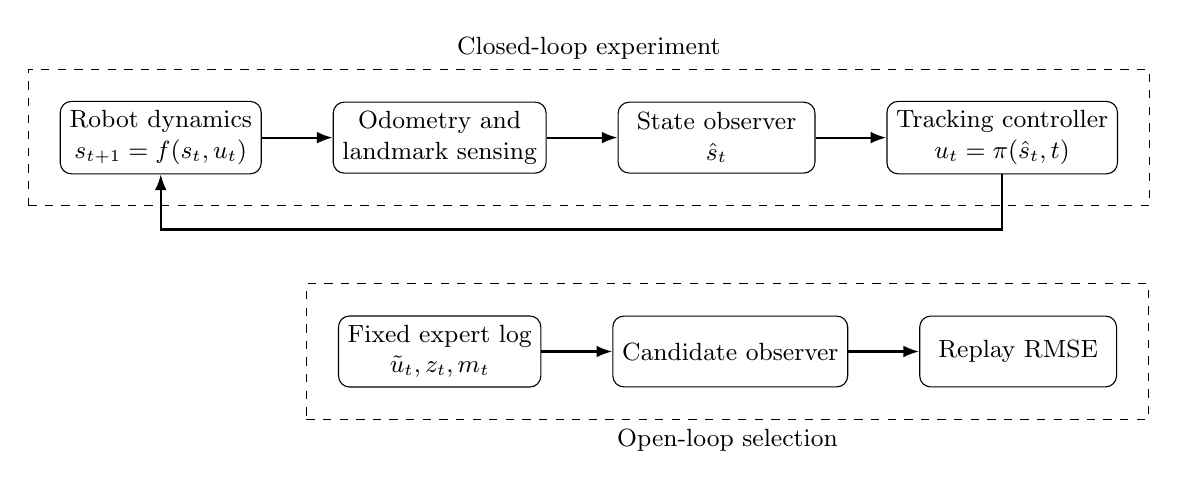
\begin{tikzpicture}[node distance=7mm and 9mm, every node/.style={font=\small}, box/.style={draw,rounded corners,align=center,minimum height=9mm,minimum width=25mm}, arr/.style={-{Latex[length=2mm]},thick}]
\node[box] (plant) {Robot dynamics\\$s_{t+1}=f(s_t,u_t)$};
\node[box,right=of plant] (sensor) {Odometry and\\landmark sensing};
\node[box,right=of sensor] (observer) {State observer\\$\hat s_t$};
\node[box,right=of observer] (controller) {Tracking controller\\$u_t=\pi(\hat s_t,t)$};
\draw[arr] (plant)--(sensor);
\draw[arr] (sensor)--(observer);
\draw[arr] (observer)--(controller);
\draw[arr] (controller.south) |- ++(0,-7mm) -| (plant.south);
\node[draw,dashed,fit=(plant)(sensor)(observer)(controller),inner sep=4mm,label=above:{Closed-loop experiment}] {};
\node[box,below=18mm of sensor] (log) {Fixed expert log\\$\tilde u_t,z_t,m_t$};
\node[box,right=of log] (replay) {Candidate observer};
\node[box,right=of replay] (score) {Replay RMSE};
\draw[arr] (log)--(replay); \draw[arr] (replay)--(score);
\node[draw,dashed,fit=(log)(replay)(score),inner sep=4mm,label=below:{Open-loop selection}] {};
\end{tikzpicture}
\caption{Open-loop replay holds inputs fixed. Closed-loop evaluation allows observer errors to change the command, the future state, and the next measurement.}
\label{fig:loop}
\end{figure}

\section{Observers}
\subsection{Classical baselines}
Dead reckoning integrates the measured odometry without exteroceptive correction. It provides a lower baseline and illustrates the effect of accumulating bias. The EKF uses the unicycle motion model and analytic range-bearing Jacobians. During a blackout, it performs prediction only. When measurements return, it applies one update for each available landmark.

\subsection{Recurrent residual observers}
Each recurrent observer wraps either dead reckoning or the EKF. The anchor first computes an analytic estimate $\bar s_t$. A recurrent model then predicts a residual $r_t$, and the final pose is
\begin{equation}
 \hat s_t = \bar s_t \oplus r_t,
\end{equation}
where $\oplus$ adds position components and wraps the heading. The input contains odometry increments, the range-bearing tuples for each landmark slot, measurement masks, an encoding of the anchor pose, and, for EKF-anchored models, the diagonal of the EKF covariance. The readout is initialized near zero so the learned observer initially behaves like its analytic anchor.

Two recurrent cores are compared. The first is a gated recurrent unit (GRU). The second is a compact diagonal state-space recurrence,
\begin{equation}
 h_t=\bar A_t h_{t-1}+\bar B_t q_t, \qquad r_t=C_t h_t,
\end{equation}
with a stable negative parameterization for the continuous-time state coefficient. In the selective version, the effective step size and input/output gates depend on the current feature vector $q_t$. In the non-selective control, these terms are fixed after training.

The six principal deployment candidates are \obs{DR}, \obs{EKF}, \obs{GRU-DR}, \obs{SSM-DR}, \obs{GRU-EKF}, and \obs{SSM-EKF}. The matched ablation additionally trains \obs{SSM-EKF-no-selectivity} and \obs{SSM-EKF-no-mask}.

\section{Evaluation method}
\subsection{Metrics}
Open-loop evaluation replays a common expert trajectory and reports position and heading RMSE. Closed-loop evaluation reports cross-track RMSE, full pose error, maximum cross-track deviation, average squared angular command, recovery after blackouts, and the fraction of steps outside a 1 m tracking tube.

For observer selection, let $q_c(o)$ be an offline score for observer $o$ in condition $c$, and let $J_c(o)$ be closed-loop cross-track RMSE. The offline choice and closed-loop oracle are
\begin{equation}
 \hat o_c=\arg\min_o q_c(o), \qquad o_c^\star=\arg\min_o J_c(o).
\end{equation}
Selection regret is
\begin{equation}
 R_c=J_c(\hat o_c)-J_c(o_c^\star).
\end{equation}
This quantity distinguishes harmless rank changes from changes that produce a meaningful tracking penalty.

In addition to pose RMSE, three controller-aware replay scores are tested. Controller-command disagreement compares the command generated from the estimated pose with the command generated from the logged true pose. Local controller-sensitivity error weights pose error by a finite-difference Jacobian of the controller. Counterfactual error replay injects the logged estimation-error sequence into a shadow closed-loop rollout. These are evaluated as alternatives, not assumed to be better in advance.

\subsection{Experimental conditions}
Table~\ref{tab:setup} summarizes the main protocol. Each observer-condition pair is evaluated with ten common random seeds. The four sweeps contain six levels each, producing 24 operating conditions. Learned observers are trained on 200 domain-randomized trajectories of 200 steps, with a separate validation set and gradient clipping.

\begin{table}[H]
\centering
\caption{Main simulation protocol.}
\label{tab:setup}
\begin{tabularx}{0.95\linewidth}{lX}
\toprule
Item & Setting \\
\midrule
Plant & Differential-drive/unicycle model, $\Delta t=0.1$ s \\
Reference & Figure-eight path, nominal speed 1.0 m/s \\
Controller & Pure pursuit, look-ahead distance 0.8 m \\
Odometry & Multiplicative slip, additive gyro bias, Gaussian noise \\
Exteroception & Range-bearing measurements to known landmarks \\
Blackout sweep & 4, 10, 16, 22, 28, 34 steps \\
Range-noise sweep & $\sigma_r=0.05,0.12,0.20,0.30,0.40,0.50$ m \\
Landmark sweep & 2, 3, 4, 5, 6, 8 active landmarks \\
Gyro-bias sweep & 0.00 to 0.25 rad/s in 0.05 increments \\
Evaluation & Ten common seeds per condition and observer \\
Training & 200 randomized trajectories, 200 steps each \\
\bottomrule
\end{tabularx}
\end{table}

\subsection{Physical-log extension}
UTIAS MRCLAM provides synchronized wheel odometry, landmark range-bearing observations, known landmark positions, and Vicon ground truth \cite{leung2011utias}. A 600 s segment of Dataset 1 Robot 1 is aligned to 6,000 time steps and contains 1,878 landmark observations. The physical-log study evaluates dead reckoning and a $3\times3$ EKF covariance grid on the original measurements. The recurrent checkpoints are also applied to an eight-landmark subset as a deliberately difficult zero-shot transfer test. A separate empirical-noise simulation samples residuals and observation timing from the physical log; it is treated as calibrated simulation, not hardware control.

\section{Results}
\subsection{Nominal closed-loop behavior}
Figure~\ref{fig:nominal_mechanism} shows the nominal trajectory and a difficult run with repeated blackouts. Dead reckoning accumulates systematic error and eventually leaves the reference. The EKF and EKF-anchored recurrent observers remain close to the path because landmark measurements periodically reset drift. During a blackout, every observer must rely on odometry; when sensing returns, the quality of the correction determines how quickly the controller recovers.

\begin{figure}[H]
\centering
\begin{subfigure}[t]{0.44\linewidth}

\includegraphics[width=\linewidth]{\figdir/fig_trajectory.png}
\caption{Closed-loop trajectories.}
\end{subfigure}\hfill
\begin{subfigure}[t]{0.53\linewidth}

\includegraphics[width=\linewidth]{\figdir/fig_timeseries.png}
\caption{Estimation error through blackouts.}
\end{subfigure}
\caption{The estimate drives the controller, so accumulated estimation error becomes tracking error.}
\label{fig:nominal_mechanism}
\end{figure}

Table~\ref{tab:nominal} gives the complete nominal comparison. The EKF is already a strong baseline. GRU-EKF obtains the lowest replay position RMSE and the lowest closed-loop cross-track RMSE. SSM-EKF is also stable but uses more angular control effort. The dead-reckoning-anchored recurrent models are the most important cautionary result: they reduce replay position error substantially compared with raw dead reckoning, but they remain much worse than the EKF in closed loop. A recurrent correction can fit a fixed trajectory without providing a sufficiently stable state for feedback.

\begin{table}[H]
\centering
\caption{Nominal performance, mean $\pm$ 95\% confidence-interval half-width over ten seeds. Lower is better.}
\label{tab:nominal}
\small
\begin{tabular}{lccccc}
\toprule
Observer & Replay pos. & Replay head. & Cross-track & Effort & Divergence \\
 & RMSE (m) & RMSE (rad) & RMSE (m) & $\overline{\omega^2}$ & fraction \\
\midrule
\obs{DR} & $1.503\pm0.200$ & $0.832\pm0.022$ & $1.045\pm0.025$ & $0.449$ & $0.260$ \\
\obs{EKF} & $0.140\pm0.009$ & $0.092\pm0.006$ & $0.212\pm0.018$ & $0.681$ & $0.004$ \\
\obs{GRU-DR} & $0.281\pm0.031$ & $0.359\pm0.087$ & $0.694\pm0.345$ & $0.914$ & $0.140$ \\
\obs{SSM-DR} & $0.325\pm0.039$ & $0.276\pm0.038$ & $0.909\pm0.498$ & $1.123$ & $0.196$ \\
\obs{GRU-EKF} & $\mathbf{0.094\pm0.012}$ & $0.093\pm0.015$ & $\mathbf{0.163\pm0.022}$ & $0.949$ & $0.000$ \\
\obs{SSM-EKF} & $0.121\pm0.018$ & $\mathbf{0.090\pm0.013}$ & $0.199\pm0.033$ & $1.052$ & $0.000$ \\
\bottomrule
\end{tabular}
\end{table}

\subsection{Degradation sweeps}
Figure~\ref{fig:sweeps} shows all four closed-loop sweeps. No learned observer is uniformly best. GRU-EKF is strongest over much of the moderate operating range, while the plain EKF becomes preferable during the longest blackouts. This behavior is physically reasonable: a learned residual can compensate for model mismatch when informative measurements are present, but it cannot create information during a complete blackout. With only two active landmarks, all methods become more sensitive to the particular geometry and visibility sequence. Under high range noise and high gyroscope bias, both EKF-anchored recurrent models remain competitive, although their relative ordering changes.

\begin{figure}[H]
\centering

\includegraphics[width=0.82\linewidth]{\figdir/fig_sweeps.png}
\caption{Closed-loop cross-track RMSE across blackout duration, measurement noise, landmark availability, and gyroscope bias. Curves show mean and 95\% confidence intervals over ten seeds.}
\label{fig:sweeps}
\end{figure}

The practical lesson is that the operating regime matters more than a single nominal ranking. A controller deployed in a warehouse with frequent visual occlusions should not be evaluated only at nominal visibility. Similarly, a system expected to experience sensor bias should include that bias in the evaluation set rather than assuming that nominal replay accuracy will extrapolate.

\subsection{Does replay RMSE select the best controller?}
Across all 144 observer-condition pairs, replay position RMSE has Spearman correlation $\rho=0.923$ and Pearson correlation $r=0.477$ with closed-loop cross-track RMSE. The high rank correlation confirms that replay RMSE is not arbitrary: it separates obviously poor observers from strong ones. The weaker magnitude correlation indicates that the size of an estimation improvement does not directly predict the size of a tracking improvement.

More importantly, the replay winner differs from the closed-loop winner in 5 of 24 conditions, or 20.8\%. Mean regret is 0.0051 m and maximum regret is 0.0347 m. The maximum is not catastrophic in this low-speed simulation, but the decision error is systematic and occurs near the top of the model ranking, where the final deployment choice is made.

\begin{figure}[H]
\centering
\begin{subfigure}[t]{0.52\linewidth}

\includegraphics[width=\linewidth]{\figdir/fig_proxy_scatter_compact.png}
\caption{Replay error versus closed-loop error.}
\end{subfigure}\hfill
\begin{subfigure}[t]{0.34\linewidth}

\includegraphics[width=\linewidth]{\figdir/fig_proxy_failures_compact.png}
\caption{Top-1 failures for offline scores.}
\end{subfigure}
\caption{Replay position RMSE gives the strongest simple baseline. A local controller-sensitivity score has fewer observed top-1 failures, but the confidence interval overlaps no improvement and its worst regret is larger.}
\label{fig:proxy}
\end{figure}

Table~\ref{tab:proxy} compares the offline scores. Heading RMSE, command disagreement, and counterfactual replay perform worse than position RMSE as top-1 selectors. Local controller-sensitivity error reduces the observed failure count to 3 of 24, but the condition-bootstrap interval for its improvement includes zero. Its maximum regret is also 0.094 m, larger than the worst regret from position RMSE. Therefore the data do not justify replacing replay position RMSE with a single controller-aware scalar. A more defensible workflow is to use replay metrics for screening and then evaluate the leading candidates in closed loop.

\begin{table}[H]
\centering
\caption{Offline selection criteria across 24 conditions.}
\label{tab:proxy}
\small
\begin{tabular}{lcccc}
\toprule
Offline score & Spearman $\rho$ & Top-1 failures & Mean regret (m) & Max regret (m) \\
\midrule
Position RMSE & $0.923$ & $5/24$ & $0.0051$ & $0.0347$ \\
Heading RMSE & $0.881$ & $19/24$ & $0.0237$ & $0.0474$ \\
Command disagreement & $0.876$ & $13/24$ & $0.0188$ & $0.1208$ \\
Local control sensitivity & $0.903$ & $3/24$ & $0.0051$ & $0.0940$ \\
Counterfactual replay & $0.842$ & $14/24$ & $0.0159$ & $0.0474$ \\
\bottomrule
\end{tabular}
\end{table}

\subsection{Compound stress}
A separate compound condition simultaneously increases slip, gyroscope bias, measurement noise, blackout duration, and landmark sparsity. Table~\ref{tab:compound} shows a clear separation between replay estimation and closed-loop utility. GRU-EKF performs best under both metrics, but SSM-EKF reduces replay position RMSE by approximately 43\% relative to the plain EKF while producing 10\% higher cross-track RMSE. This is the clearest pairwise example of objective mismatch in the study: the learned residual improves the fixed-log estimate but does not improve control.

\begin{table}[H]
\centering
\caption{Compound-stress evaluation over ten seeds.}
\label{tab:compound}
\small
\begin{tabular}{lccc}
\toprule
Observer & Replay position (m) & Closed-loop pose (m) & Cross-track (m) \\
\midrule
\obs{DR} & $3.289\pm0.382$ & $4.818\pm0.030$ & $2.528\pm0.014$ \\
\obs{EKF} & $0.829\pm0.066$ & $1.467\pm0.358$ & $1.324\pm0.094$ \\
\obs{GRU-EKF} & $\mathbf{0.447\pm0.049}$ & $\mathbf{1.222\pm0.422}$ & $\mathbf{1.052\pm0.326}$ \\
\obs{SSM-EKF} & $0.472\pm0.044$ & $1.496\pm0.350$ & $1.459\pm0.156$ \\
\obs{SSM-DR} & $0.798\pm0.099$ & $5.734\pm1.419$ & $4.228\pm1.360$ \\
\bottomrule
\end{tabular}
\end{table}

\subsection{Matched architecture ablation}
The original architecture comparison could have been misleading if recurrence design and anchor quality were changed at the same time. The final ablation keeps the EKF anchor fixed and changes only selectivity or mask access. Figure~\ref{fig:robustness}a shows that the three models are nearly tied at nominal conditions. The non-selective model is better during long blackouts and with two landmarks, while the selective model is better under high gyroscope bias. Removing the explicit mask does not consistently cause failure because zero-filled measurement channels and the EKF covariance still provide indirect information about measurement availability.

This result changes the interpretation of the project. Selectivity is not the main reason the learned observer remains stable. The EKF anchor is the load-bearing component. Selectivity changes the bias-robustness trade-off and may help in some regimes, but it is not a universal stability mechanism.

\begin{figure}[H]
\centering
\begin{subfigure}[t]{0.44\linewidth}

\includegraphics[width=\linewidth]{\figdir/fig_matched_ekf_ablation.png}
\caption{Same-anchor selectivity and mask ablation.}
\end{subfigure}\hfill
\begin{subfigure}[t]{0.44\linewidth}

\includegraphics[width=\linewidth]{\figdir/fig_training_seed_robustness.png}
\caption{Three SSM-EKF training initializations.}
\end{subfigure}
\caption{Architecture conclusions become more cautious after controlling the analytic anchor and training initialization.}
\label{fig:robustness}
\end{figure}

\subsection{Training initialization and controller dependence}
The SSM-EKF model was trained with three independent initialization seeds. Nominal mean cross-track RMSE ranges only from 0.189 to 0.199 m, but long-blackout performance ranges from 0.231 to 0.336 m. High-noise and high-bias conditions also show visible variation. A single training run is therefore adequate for demonstrating the method, but not for making a strong claim about difficult regimes.

The controller-sensitivity experiment replaces pure pursuit with the Kanayama controller while preserving the plant, sensing conditions, checkpoints, actuator limits, and five matched evaluation seeds. The closed-loop oracle changes in 8 of 24 conditions. Replay position RMSE selects the wrong Kanayama observer in 7 of 24 conditions, with maximum regret 0.092 m. The seed-bootstrap interval is wide because only five seeds were used, so this is reported as a secondary analysis. Even with that limitation, it confirms that observer quality is partly controller-dependent.

\subsection{Physical-log localization}
The 600 s MRCLAM Robot 1 trajectory is shown in Figure~\ref{fig:external}. Dead reckoning reaches 3.392 m position RMSE, while the best covariance setting in the evaluated EKF grid reaches 1.357 m. This confirms that the classical estimator and data loader work on physical odometry and range-bearing measurements rather than only in the synthetic environment.

The zero-shot recurrent checkpoints are less successful. On an eight-landmark subset, the learned EKF residuals improve position error modestly relative to dead reckoning but worsen heading error. The fixed ordered landmark-slot representation was trained on one simulated map and does not generalize cleanly to a new landmark arrangement. The next technical step is to use a permutation-invariant set representation and train across randomized maps.

\begin{figure}[H]
\centering
\begin{subfigure}[t]{0.40\linewidth}

\includegraphics[width=\linewidth]{\figdir/fig_controller_sensitivity.png}
\caption{Controller sensitivity.}
\end{subfigure}\hfill
\begin{subfigure}[t]{0.48\linewidth}

\includegraphics[width=\linewidth]{\figdir/fig_mrclam_real_trajectory.png}
\caption{MRCLAM physical-log trajectory.}
\end{subfigure}
\caption{Secondary checks outside the main pure-pursuit simulation. The controller analysis uses five matched seeds. The MRCLAM result uses physical odometry, range-bearing measurements, known landmarks, and Vicon ground truth.}
\label{fig:external}
\end{figure}

\begin{table}[H]
\centering
\caption{Physical-log localization on 600 s of MRCLAM Robot 1.}
\label{tab:mrclam}
\begin{tabular}{lcc}
\toprule
Method & Position RMSE (m) & Heading RMSE (rad) \\
\midrule
Dead reckoning, 15 landmarks & $3.392$ & $1.662$ \\
Best EKF grid point, 15 landmarks & $\mathbf{1.357}$ & $\mathbf{0.850}$ \\
GRU-EKF zero-shot, 8-landmark subset & $2.597$ & worse than matched DR baseline \\
SSM-EKF zero-shot, 8-landmark subset & $2.625$ & worse than matched DR baseline \\
\bottomrule
\end{tabular}
\end{table}

\section{Discussion}
\subsection{What worked}
The project successfully assembled a complete autonomy loop rather than evaluating estimation alone. The plant, intermittent sensing, state observer, and trajectory controller interact at every step. This made it possible to answer the central question directly. The EKF-anchored residual observers were the strongest learned designs because the analytic recursion continued to provide a reasonable pose and uncertainty estimate when the recurrent correction was imperfect. The GRU-EKF observer improved nominal tracking and several noisy or biased regimes without sacrificing stability.

The controlled degradation sweeps were also valuable. They showed that the same observer can be strong under model mismatch and less useful under information loss. High noise and high bias leave measurements available but imperfect, which gives a learned residual something to correct. Long blackouts remove information entirely, so the plain EKF prediction can be as good as or better than an additional learned correction.

Finally, the corrected selection analysis produced a more useful result than a simple architecture ranking. It quantified when replay selection changes the deployment decision and how costly that decision is. This is directly relevant to how an engineer would choose a model for a robot.

\subsection{What did not work as expected}
The strongest initial expectation was that selective recurrence and explicit measurement-mask input would be essential for closed-loop stability. The matched EKF-anchor ablation did not support that general claim. Selectivity helped under high gyroscope bias but hurt during long blackouts and sparse sensing. The mask-free model remained stable because other inputs carried redundant information about measurement availability. This was an important correction: the analytic anchor, not the recurrence variant by itself, was the dominant stabilizing choice.

The controller-aware offline metrics also did not provide a complete replacement for pose RMSE. Instantaneous command disagreement can over-penalize harmless local corrections and under-represent accumulated heading drift. Local sensitivity reduced the observed top-1 failures, but the uncertainty was too large to claim a reliable improvement. Counterfactual replay was still based on an injected logged error sequence and could not reproduce the full state-distribution shift of a real closed-loop rollout.

The physical-log experiment exposed a representation problem. A fixed ordered list of landmark slots is convenient in one map but fragile when landmarks are reordered or the map size changes. The next version should encode the set of current innovations independently of landmark ordering, pool them into a fixed-dimensional summary, and train over many randomized maps.

\subsection{Limitations}
The main study is simulation-only, uses one differential-drive model, and focuses on a figure-eight path. The recurrent observers were trained on 200 trajectories, and only the SSM-EKF model has three independent training initializations. The Kanayama comparison uses five evaluation seeds. MRCLAM provides physical sensing but not a hardware closed-loop deployment of the learned observers. The selected control speeds are modest, so the absolute regret values are smaller than they could be on a faster or less stable platform.

These limitations do not invalidate the central result, because replay and closed-loop evaluations are paired within the same controlled environment. They do limit generalization. A stronger follow-up would use randomized maps and trajectories, more training seeds, controller-gain sweeps, multiple MRCLAM robots, and a ROS/Gazebo or hardware experiment with real timing and actuator constraints.

\section{Reproducibility and repository organization}
The final repository is organized so that a grader can reproduce the best result without searching through paper drafts or intermediate files. The root \texttt{README.md} contains installation and execution instructions. \texttt{requirements.txt} and \texttt{environment.yml} define the software environment. The \texttt{src/ssm\_obs} package contains dynamics, sensing, observers, controllers, metrics, plotting, and MRCLAM loading. The \texttt{scripts} directory contains training and evaluation entry points. Bundled checkpoints and audited reference JSON files are stored under \texttt{results}. Unit tests cover controller-aware metrics and MRCLAM parsing.

Running \texttt{bash reproduce.sh} executes the regression tests, performs a fresh closed-loop smoke experiment, verifies the reported result files, and checks the report and video assets. Running \texttt{bash reproduce.sh --full} reruns the complete simulation study from the bundled checkpoints. Raw MRCLAM data are not included because they are externally hosted, but a downloader and exact evaluation command are provided.

\section{Conclusion}
This project tested whether the observer with the lowest replay estimation error is also the best observer for closed-loop robot control. In a differential-drive tracking problem with intermittent landmark sensing, replay position RMSE was strongly correlated with cross-track error but selected a different closed-loop winner in 5 of 24 operating conditions. The most reliable learned observers retained an EKF anchor and learned only a residual correction. Selective recurrence was helpful in some regimes but was not a universal source of stability, and controller-aware replay scores did not remove the need for closed-loop testing.

The resulting engineering recommendation is straightforward. Use open-loop replay to remove clearly poor observers, then run the leading candidates in a small, representative set of closed-loop conditions that covers the expected sensor failures and controller settings. For a robot, the state estimate is only useful through the behavior it produces.

\clearpage
\begin{thebibliography}{99}
\small
\bibitem{thrun2005probabilistic} S. Thrun, W. Burgard, and D. Fox, \emph{Probabilistic Robotics}. MIT Press, 2005.
\bibitem{coulter1992pure} R. C. Coulter, ``Implementation of the pure pursuit path tracking algorithm,'' Carnegie Mellon University Robotics Institute, Tech. Rep. CMU-RI-TR-92-01, 1992.
\bibitem{kanayama1990stable} Y. Kanayama, Y. Kimura, F. Miyazaki, and T. Noguchi, ``A stable tracking control method for an autonomous mobile robot,'' in \emph{Proc. IEEE ICRA}, 1990, pp. 384--389.
\bibitem{ha2016backprop} T. Haarnoja, A. Ajay, S. Levine, and P. Abbeel, ``Backprop KF: Learning discriminative deterministic state estimators,'' in \emph{Advances in Neural Information Processing Systems}, 2016.
\bibitem{karl2017dvbf} M. Karl, M. Soelch, J. Bayer, and P. van der Smagt, ``Deep variational Bayes filters,'' in \emph{International Conference on Learning Representations}, 2017.
\bibitem{becker2019rkn} P. Becker et al., ``Recurrent Kalman networks: Factorized inference in high-dimensional deep feature spaces,'' in \emph{International Conference on Machine Learning}, 2019.
\bibitem{jonschkowski2018dpf} R. Jonschkowski, D. Rastogi, and O. Brock, ``Differentiable particle filters: End-to-end learning with algorithmic priors,'' in \emph{Robotics: Science and Systems}, 2018.
\bibitem{revach2022kalmannet} G. Revach et al., ``KalmanNet: Neural network aided Kalman filtering for partially known dynamics,'' \emph{IEEE Transactions on Signal Processing}, vol. 70, pp. 1532--1547, 2022.
\bibitem{rubanova2019latentode} Y. Rubanova, R. T. Q. Chen, and D. Duvenaud, ``Latent ordinary differential equations for irregularly-sampled time series,'' in \emph{Advances in Neural Information Processing Systems}, 2019.
\bibitem{gu2022s4} A. Gu, K. Goel, and C. R\'e, ``Efficiently modeling long sequences with structured state spaces,'' in \emph{International Conference on Learning Representations}, 2022.
\bibitem{gu2024mamba} A. Gu and T. Dao, ``Mamba: Linear-time sequence modeling with selective state spaces,'' in \emph{Conference on Language Modeling}, 2024.
\bibitem{lambert2020objective} N. Lambert, B. Amos, O. Yadan, and R. Calandra, ``Objective mismatch in model-based reinforcement learning,'' in \emph{Conference on Learning for Dynamics and Control}, 2020, pp. 761--770.
\bibitem{leung2011utias} K. Y. K. Leung, Y. Halpern, T. D. Barfoot, and H. H. T. Liu, ``The UTIAS multi-robot cooperative localization and mapping dataset,'' \emph{The International Journal of Robotics Research}, vol. 30, no. 8, pp. 969--974, 2011.
\end{thebibliography}
\end{document}
